\documentclass[11pt]{article}
\usepackage{latexsym}
\usepackage{amsmath}
\usepackage{amssymb}
\usepackage{amsthm}
\usepackage{epsfig}
% \usepackage[tight]{subfigure}
\usepackage{bm}
\usepackage{graphicx}
\usepackage{caption}
\usepackage{subcaption}
\usepackage{float}

\usepackage{amsmath}

\DeclareMathOperator*{\minimize}{min}
\DeclareMathOperator*{\maximize}{max}

\usepackage{algorithm}
 %on linux you may need to run sudo apt-get install texlive-full to install algorithm.sys
\usepackage{algorithmic}

\usepackage{verbatim}

\newcommand{\handout}[5]{
  \noindent
  \begin{center}
  \framebox{
    \vbox{
      \hbox to 5.78in { {#1} \hfill #2 }
      \vspace{4mm}
      \hbox to 5.78in { {\Large \hfill #5  \hfill} }
      \vspace{2mm}
      \hbox to 5.78in { {\em #3 \hfill #4} }
    }
  }
  \end{center}
  \vspace*{4mm}
}

\newcommand{\lecture}[5]{\handout{#1}{#2}{#3}{#4}{#5}}
\newcommand{\collision}[0]{\mathrm{collision}}
\newcommand{\nocollision}[0]{\overline{\collision}}

\newcommand*{\QED}{\hfill\ensuremath{\square}}

\newcommand{\argmax}[1]{\underset{#1}{\operatorname{arg}\,\operatorname{max}}\;}
\newcommand{\argmin}[1]{\underset{#1}{\operatorname{arg}\,\operatorname{min}}\;}

\newtheorem{theorem}{Theorem}
\newtheorem{corollary}[theorem]{Corollary}
\newtheorem{lemma}[theorem]{Lemma}
\newtheorem{observation}[theorem]{Observation}
\newtheorem{proposition}[theorem]{Proposition}
\newtheorem{definition}[theorem]{Definition}
\newtheorem{claim}[theorem]{Claim}
\newtheorem{fact}[theorem]{Fact}
\newtheorem{assumption}[theorem]{Assumption}
\newtheorem{note}[theorem]{Note}

% 1-inch margins, from fullpage.sty by H.Partl, Version 2, Dec. 15, 1988.
\topmargin 0pt
\advance \topmargin by -\headheight
\advance \topmargin by -\headsep
\textheight 8.9in
\oddsidemargin 0pt
\evensidemargin \oddsidemargin
\marginparwidth 0.5in
\textwidth 6.5in

\parindent 0in
\parskip 1.5ex
%\renewcommand{\baselinestretch}{1.25}

\begin{document}

\lecture{Statistical Techniques in Robotics (16-831, S21)}{Lecture \#21
  (Wednesday, April 21)}{Lecturer: Kris Kitani}{Scribes: Andy Wei, Yi-Chun Chen}{Policy Gradient Methods, Actor-Critic}

\section{Review}
In the last lecture, we talked model-free value-based control, value function approximation, and an introduction to policy-based control. In this note, we will cover policy gradient method, a type of policy-based control method, and actor-critic, a hybrid of policy-based and value based control. In this section, we will review model-free control algorithm and value function approximation.
\subsection{Model-Free Control}
Model-free control aims to estimate the optimal policy without knowing the exact environment model; that is, the algorithm uses sampled value function to improve policy. Fig \ref{fig:model_free} shows the pipeline of model-free control. One can use any model-free prediction methods, e.g. TD Prediction, Monte-Carlo Prediction, when doing policy evaluation. We only listed the Monte-Carlo control in section 1.1.1 to let this note be concise. 
\begin{figure}[H]
    \centering
    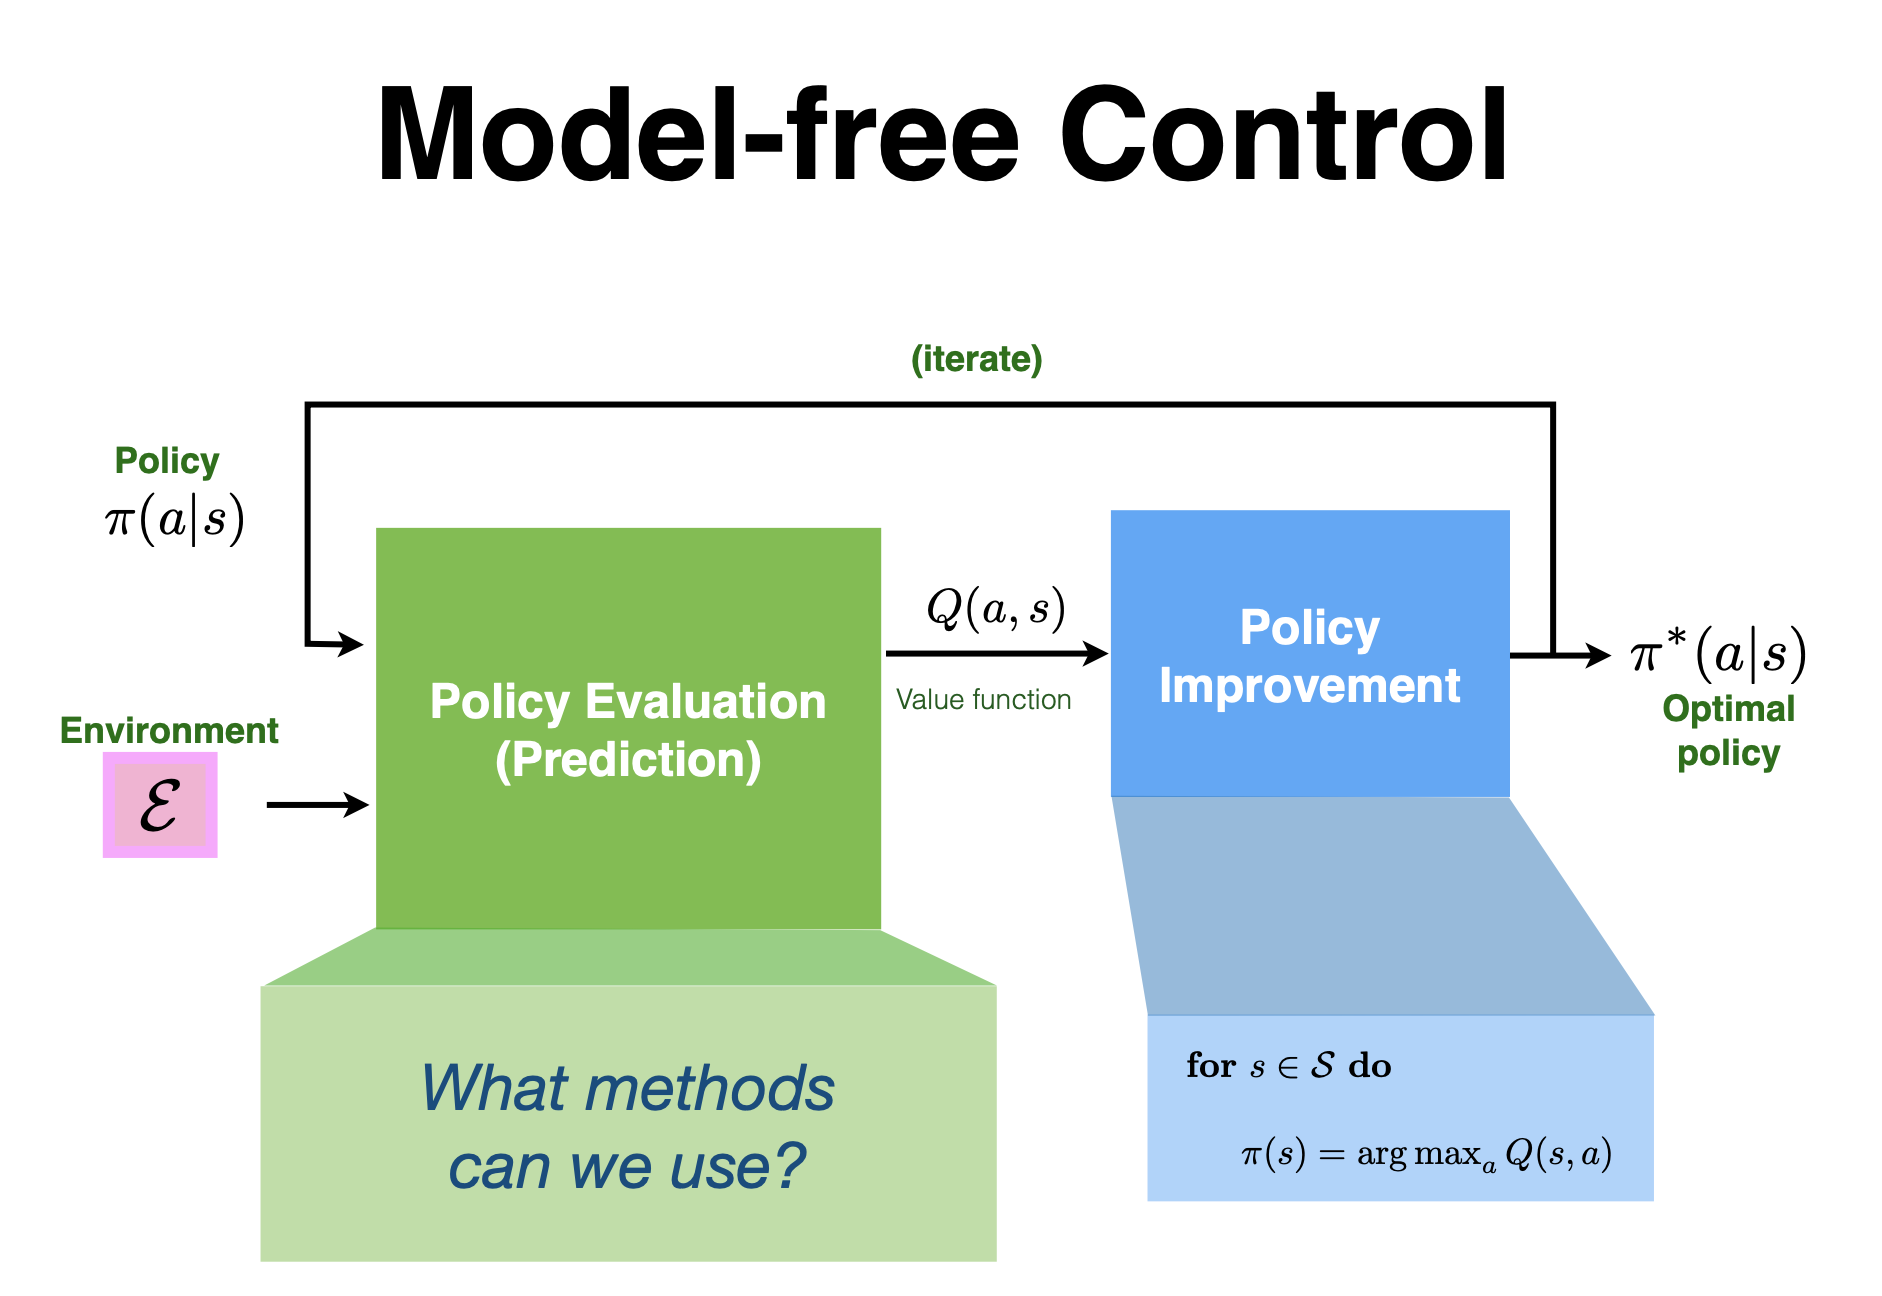
\includegraphics[scale=0.2]{images/model-free.png}
    \caption{Model-Free Control Pipeline}
    \label{fig:model_free}
\end{figure}
\subsubsection{Model-Free Control Methods Example: Monte-Carlo Control}
The below listed the Monte-Carlo Control algorithm as Algorithm~\ref{algo:mc}. Line 4 and line 5 are the monte-carlo prediction. Line 6 is the epsilon greedy policy, which forces the algorithm to explore random policy with probability $\epsilon$. 
\begin{algorithm}[H]
\caption{MC Control(\pi_{\epsilon}, \epsilon, \alpha)}
\label{algo:mc}
\begin{algorithmic}[1]
\FOR{$e=0,\;\cdots,\;E$}
\STATE $\{ s^{(t)}, a^{(t)}, r^{(t)} \}_{t=0}^T$ \sim $\mathcal{\epsilon} | \pi_{\epsilon}$ 
\FOR{$t=0,\;\cdots,\;T$}
\STATE $Q( a^{(t)}, s^{(t)}) \leftarrow Q( a^{(t)}, s^{(t)}) + \alpha [G^{(t)} - Q( a^{(t)}, s^{(t)})]$ 

\STATE $a^* = \text{argmax}_a Q(a, s^{(t)})$
\STATE $\pi_\epsilon (a|s^{(t)}) \leftarrow \frac{\epsilon}{\mathcal{A}(s^{(t)})} + \textbf{1}[a = a^*](1 - \epsilon) ~ \forall a$
\ENDFOR
\ENDFOR
\end{algorithmic}
\end{algorithm}

\subsection{Value Function Approximation}
With finite state and action space, previously we only talked about a tabular value function. However, it is infeasible to use a tabular value function when the state or action space is infinite, as it may require infinite memory to store values for all combination of states and actions; this is where the value function approximation helps. The value function approximation aims to learn a function $V_\theta (s)$ that approximates the real value function $V(s)$ using some parameter $\theta$, where s is the input state. Thus, the objectives will be finding a the optimal $\theta$
$$\hat{\theta} = \text{argmin}_\theta \mathbb{E}_p [(V(s) - V_\theta (s))^2]$$
where p is the state visitation distribution. The solution can be found using stochastic gradient descent
$$\nabla_\theta L_\theta = -(V(s) - V_\theta (s)) \frac{\partial}{\partial \theta} V_\theta(s)$$
However, as we don't know the value function V(s), we use the estimate of the value function
$$V(s) = \mathbb{E}[G^{(t)}] \approx G^{(t)}$$
,with such estimation being done by model-free prediction methods we've covered, e.g. Monte-Carlo, TD.
Similarly, the Q-value can be approximated using $Q_\theta (s, a)$. Such approximator can be linear function, neural networks, or even deep neural networks. 

\section{Summary}
\subsection{Policy Gradient Methods}
Policy gradient methods is a type of reinforcement learning algorithm that directly learns the policy without estimating the value function. The goal of policy gradient methods is to find the policy parameters that maximizes the expected return
\begin{align*}
    \hat{\theta} & = \argmax{\theta} \mathbb{E}_{p_\theta(\zeta)}\left[\sum_{t=0}^Tr^{(t)}\right] \\
    & = \argmax{\theta} J(\theta)
\end{align*},
where 
\begin{align*}
    & p_\theta(\zeta) = p(s^{(0)})\Pi_{t=0}^T\pi_\theta(a^{(t)}|s^{(t)})p(s^{(t+1)}|s^{(t)}, a^{(t)}) \\
    & \zeta  = \{s^{(0)}, a^{(0)}, s^{(1)}, a^{(1)}, ..., s^{(T)}, a^{(T)}\} \\
    & r^{(t)} \triangleq r(s^{(t+1)}, a^{(t)}, s^{(t)})
\end{align*}

\subsubsection{Gradient Ascent}

The way to find the policy that maximizes the expected return is \emph{gradient ascent}. First, we make a linear approximation of the objective function with quadratic regularization.
\begin{align*}
    \hat{\theta} = \argmax{\theta}\{\alpha(J(\theta^{'})+\langle\theta-\theta^{'}, \nabla_\theta^{'}J(\theta^{'})\rangle - \frac{1}{2}||\theta-\theta^{'}||^2)\}
\end{align*}
Then, we want to solve for the parameters that optimizes the Lagrangian, and we can get the parameters update equation.
\begin{align*}
    & \nabla_\theta\{\alpha(J(\theta^{'})+\langle\theta-\theta^{'}, \nabla_\theta^{'}J(\theta^{'})\rangle - \frac{1}{2}||\theta-\theta^{'}||^2)\} = 0 \\
    \Rightarrow & \;\alpha\nabla_{\theta^{'}}J(\theta^{'}) - \theta + \theta^{'} = 0 \\
    \Rightarrow & \;\theta \leftarrow \theta^{'} + \alpha \nabla_{\theta^{'}}J(\theta^{'})
\end{align*}

Recall that
\begin{align*}
    J(\theta)&  = \mathbb{E}_{p_\theta(\zeta)}\left[\sum_{t=0}^Tr^{(t)}\right] = \int_\zeta p_\theta(\theta)r(\zeta)d\zeta, \;\;\;\;\; r(\zeta) = \sum_{t=0}^Tr^{(t)}
\end{align*}
Then, we can start to compute the gradient.
\begin{align*}
    \nabla_\theta J(\theta) & = \nabla_\theta \int_\theta p_\theta(\theta)r(\zeta)d\zeta \;\;\;\;\; \text{\footnotesize{, by definition}}\\
    & = \int_\theta \nabla_\theta p_\theta(\theta)r(\zeta)d\zeta \;\;\;\;\; \text{\footnotesize{, linearity of gradient}}\\
    & = \int_\theta p_\theta \frac{\nabla_\theta p_\theta(\theta)}{p_\theta}r(\zeta)d\zeta \;\;\;\;\; \text{\footnotesize{, multiply by one}}\\
    & = \int_\theta p_\theta \nabla_\theta \ln p_\theta(\theta)r(\zeta)d\zeta \;\;\;\;\; \text{\footnotesize{, derivative of log}}
\end{align*}

Next, we want to decompose the term $\nabla_\theta \ln p_\theta(\theta)$ and bring it back to the gradient $\nabla_\theta J(\theta)$.
\begin{align*}
    \nabla_\theta \ln p_\theta(\theta) & = \nabla_\theta \left[ \ln p(s^{(0)}) + \sum_{t=1}^T \ln \pi_\theta(a^{(t)}|s^{(t)}) + \ln p(s^{(t+1)}|s^{(t)}, a^{(t)}) \right] \\
    & = \nabla_\theta \left[ \sum_{t=1}^T \ln \pi_\theta(a^{(t)}|s^{(t)})  \right]\;\;\;\;\; \text{\footnotesize{, only policy is dependent on theta}} \\
    \nabla_\theta J(\theta) & = \int_\theta p_\theta \nabla_\theta \ln p_\theta(\theta)r(\zeta)d\zeta \\
    & = \int_\theta p_\theta \nabla_\theta \Bigg(\sum_{t=1}^T \ln \pi_\theta(a^{(t)}|s^{(t)})\Bigg) r(\zeta)d\zeta \\
    & = \mathbb{E}_{p_\theta}\left[ \Bigg( \sum_{t=1}^T \nabla_\theta \ln \pi_\theta(a^{(t)}|s^{(t)}) \Bigg) \Bigg( \sum_{t=1}^T r^{(t)} \Bigg) \right]
\end{align*}

We consider the term $\nabla_\theta \ln \pi_\theta(a^{(t)}|s^{(t)})$ eligibility vector. Intuitively, it is a weighted sensitivity of the policy to change in parameter. Since $\nabla_\theta \ln \pi_\theta(a^{(t)}|s^{(t)}) = \frac{\nabla_\theta \pi_\theta(a^{(t)}|s^{(t)})}{\pi_\theta(a^{(t)}|s^{(t)})}$, one can interpret that low probability actions have bigger gradient while high probability actions have smaller gradient. And we consider the other term $r(\zeta) = \sum_{t=1}^T r^{(t)}$ episodic return. The intuition is it is goodness of the current policy. Large reward (good trajectory) means bigger gradient while small reward (bad trajectory) means small gradient.

It is impossible to sum over all possible trajectories to compute the expectation, so we can use approximation, e.g. Monte-Carlo estimate. Therefore, we can obtain that

\begin{align*}
    \nabla_\theta J(\theta) & = \mathbb{E}_{p_\theta}\left[ \Bigg( \sum_{t=1}^T \nabla_\theta \ln \pi_\theta(a^{(t)}|s^{(t)}) \Bigg) \Bigg( \sum_{t=1}^T r^{(t)} \Bigg) \right] \\
    & = \frac{1}{N}\sum_{n=1}^N \Bigg( \sum_{t=1}^T \nabla_\theta \ln \pi_\theta(a^{(n, t)}|s^{(n, t)}) \Bigg) \Bigg( \sum_{t=1}^T r^{(n, t)} \Bigg)
\end{align*}

\subsubsection{Monte-Carlo Policy Gradient and Reinforce}
Let's look at the algorithm of Monte-Carlo policy gradient.
\begin{algorithm}[H]
\caption{MC-Policy-Gradient}
\begin{algorithmic}[1]
\FOR{$e=1,\;\cdots,\;E$}
\STATE $\{s^{(t)}, a^{(t)}, r^{(t)}\}_{t=0}^T \sim \mathcal{E}|\pi_\theta$
\STATE $G^{(0)} = \sum_{t=0}^T r^{(t)}$ 
\FOR{$t=0,\;\cdots,\;T$}
\STATE $\theta \leftarrow \theta + \alpha \Big( \nabla_\theta \log \pi_\theta (a^{(t)}|s^{(t)}) \Big) \Big( G^{(0)} \Big) $
\ENDFOR
\ENDFOR
\RETURN $\pi_\theta$
\end{algorithmic}
\end{algorithm}

A problem of the gradient is that Monte Carlo estimate has high variance. There are two ways to reduce variance of policy gradient. The first one is to enforce causality. The original gradient involves the reward of entire trajectory. However, the update to the policy at time t should only depend on future reward. Therefore, we can write the gradient as
\begin{align*}
    \nabla_\theta J(\theta) & \approx \frac{1}{N}\sum_{n=1}^N \Bigg( \sum_{t=0}^T \nabla_\theta \ln \pi_\theta(a^{(n, t)}|s^{(n, t)}) \Bigg) \Bigg( \sum_{t=1}^T r^{(n, t)} \Bigg) \\
    & \approx \frac{1}{N}\sum_{n=1}^N \Bigg( \sum_{t=0}^T \nabla_\theta \ln \pi_\theta(a^{(n, t)}|s^{(n, t)}) \Bigg) \Bigg( \sum_{t^{'}=t}^T r^{(n, t^{'})} \Bigg)
\end{align*}

The other way is to remove gradient bias with a baseline offset. We can observe that large rewards results in large gradient variance, so we can adjust the gradient by subtracting some offset b, and the expected reward still stays the same.
\begin{align*}
    \nabla_\theta J(\theta) & = \int_\theta p_\theta(\zeta) \nabla_\theta \ln p_\theta(\theta)[r(\zeta)-b]d\zeta \\
\end{align*}
Below shows that offset will not change the expected gradient.
\begin{align*}
    \nabla_\theta J(\theta) & = \int_\theta p_\theta(\zeta) \nabla_\theta \ln p_\theta(\theta)[r(\zeta)-b]d\zeta \\
    & = \int_\theta p_\theta(\zeta) \nabla_\theta \ln p_\theta(\theta)r(\zeta)d\zeta - \int_\theta p_\theta(\zeta) \nabla_\theta \ln p_\theta(\theta)bd\zeta \\
    & = \int_\theta p_\theta(\zeta) \nabla_\theta \ln p_\theta(\theta)r(\zeta)d\zeta - \int_\theta p_\theta(\zeta) \frac{\nabla_\theta p_\theta(\zeta)}{p_\theta(\zeta)}bd\zeta \\
    & = \int_\theta p_\theta(\zeta) \nabla_\theta \ln p_\theta(\theta)r(\zeta)d\zeta - b\nabla_\theta \int_\theta p_\theta(\zeta) d\zeta \\
    & = \int_\theta p_\theta(\zeta) \nabla_\theta \ln p_\theta(\theta)r(\zeta)d\zeta - b\nabla_\theta(1) \\
    & = \int_\theta p_\theta(\zeta) \nabla_\theta \ln p_\theta(\theta)r(\zeta)d\zeta - 0
\end{align*}

It is worth noting that in the episodic reinforce algorithm \cite{williams1992simple}, the policy parameter updates is subtracting a baseline.
\begin{algorithm}[H]
\caption{Episodic Reinforce($\pi_theta, \alpha$)}
\begin{algorithmic}[1]
\FOR{$e=1,\;\cdots,\;E$}
\STATE $\{s^{(t)}, a^{(t)}, r^{(t)}\}_{t=0}^T \sim \mathcal{E}|\pi_\theta$
\STATE $G^{(0)} = \sum_{t=0}^T r^{(t)}$ 
\FOR{$t=0,\;\cdots,\;T$}
\STATE $\theta \leftarrow \theta + \alpha [G^{(0)}-b] \nabla_\theta \log \pi_\theta (a^{(t)}|s^{(t)}) $
\ENDFOR
\ENDFOR
\RETURN $\pi_\theta$
\end{algorithmic}
\end{algorithm}

We can interpret REINFORCE with REward Increment = Non-negative Factor $\times$ Offset Reinforcement $\times$ Characteristic Eligibility.

\begin{center}
    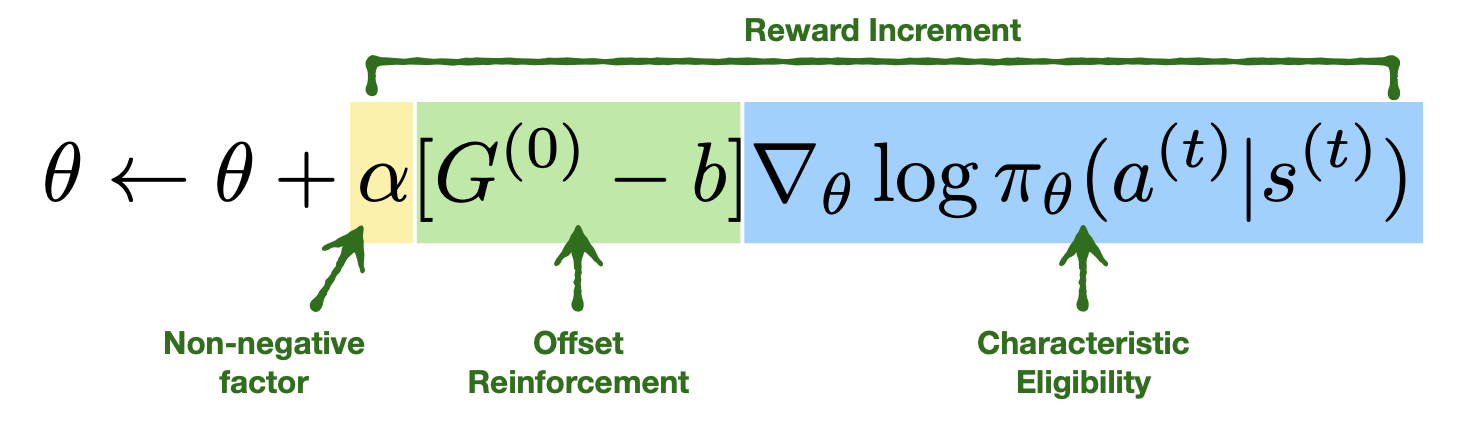
\includegraphics[width=.5\linewidth]{images/Reinforce.png}
\end{center}

To sum, adding baseline reduces the variance. As the variance is reduced, you don't need to sample as many trajectories to estimate the return. From the figure\cite{sutton2018reinforcement}, you can see that reinforce with baseline converges faster.

\begin{center}
    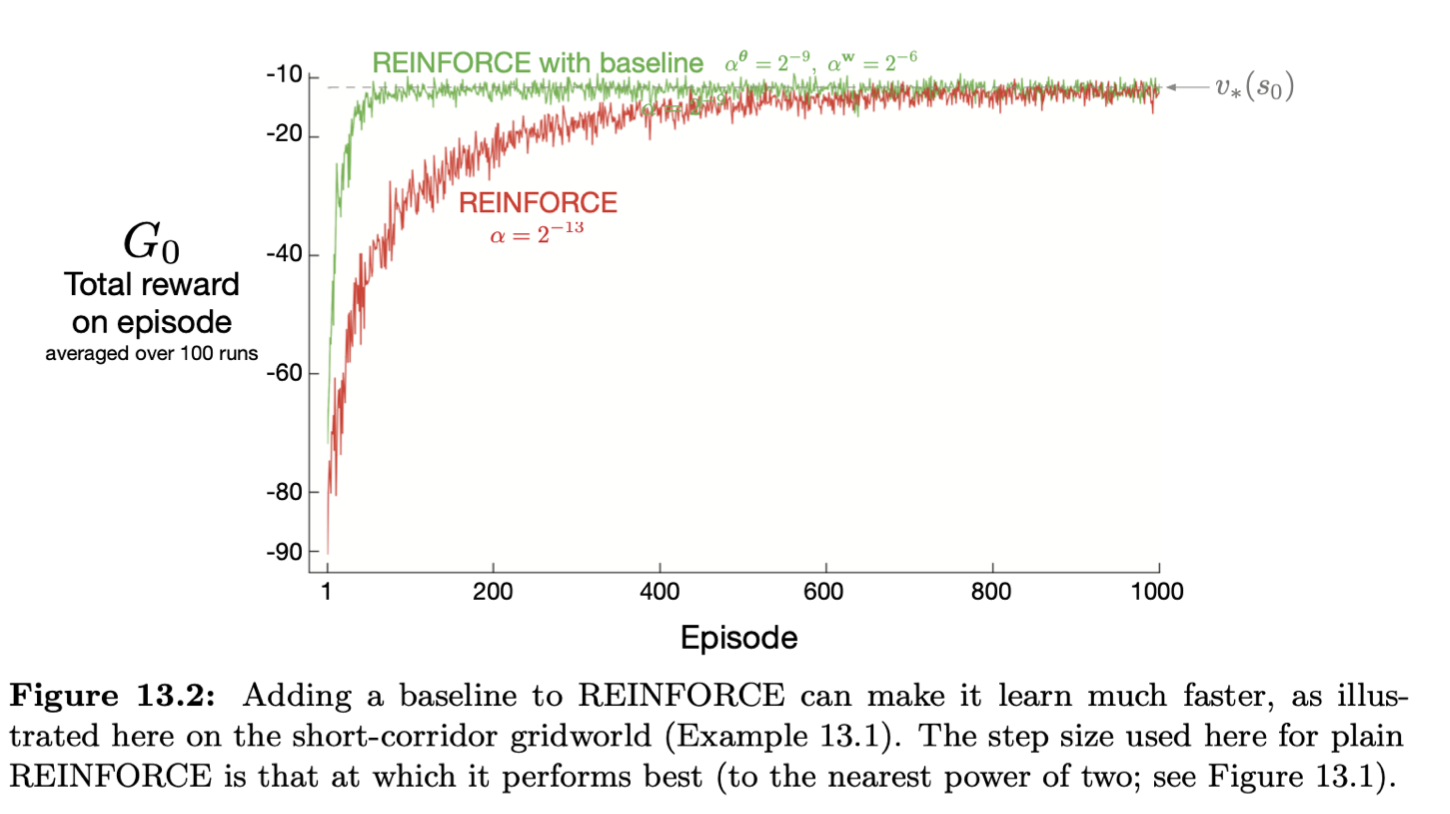
\includegraphics[width=.5\linewidth]{images/Reinforce_baseline.png}
\end{center}

\subsubsection{Policy Gradient}
Putting the two modifications above together, we get the policy gradient algorithm.
\begin{algorithm}[H]
\caption{Policy Gradient($\pi_\theta, \alpha, b$)}
\begin{algorithmic}[1]
\FOR{$e=1,\;\cdots,\;E$}
\STATE $\{s^{(t)}, a^{(t)}, r^{(t)}\}_{t=0}^T \sim \mathcal{E}|\pi_\theta$
\FOR{$t=0,\;\cdots,\;T$}
\STATE $G^{(t)} = \sum_{i=t}^T r^{(i)}$  \hfill (1) Enforce causality
\STATE $\theta \leftarrow \theta + \alpha [G^{(t)}-b] \nabla_\theta \log \pi_\theta (a^{(t)}|s^{(t)}) $ \hfill (2) Subtract baseline
\ENDFOR
\ENDFOR
\RETURN $\pi_\theta$
\end{algorithmic}
\end{algorithm}

Lastly, we list down the pros and cons of policy gradient methods.

Pros:
\begin{itemize}
    \item Doesn't require model and learns from interaction
    \item Effective for high-dimensional or continuous action spaces (all methods so far assumed finite action space)
    \item Can encode prior knowledge when designing policy architecture
    \item Finds the optimal stochastic policy and naturally explores due to stochasticity
\end{itemize}

Cons:
\begin{itemize}
    \item Gradient is typically high variance and leads to slow convergence
    \item Small step size leads to slow convergence
    \item Typically converge to local minima instead of global minima
    \item Exploding or zero gradient
\end{itemize}

\subsection{Actor Critic}
In the policy gradient, we have
$$\nabla_\theta J(\theta) = \mathbb{E}_{p_\theta} [(\sum_{t=1}^T \nabla_\theta \ln \pi_\theta (a^{(t)} | s^{(t)}))(\sum_{t=1}^T r^{(t)})]$$
However, the $\sum_{t=1}^T r^{(t)}$ requires full-episode to compute. To prevent from such issues, Actor-Critic method uses model-free prediction for the return value estimator. For continuous state, we can further use function approximation for such estimate. Thus we have
$$\nabla_\theta J(\theta) = \mathbb{E}_{p_\theta} [(\sum_{t=1}^T \nabla_\theta \ln \pi_\theta (a^{(t)} | s^{(t)}))Q_\phi (a^{(t)}, s^{(t)})]$$
where $G_\phi$ is function approximation of the return value parameterize by $\phi$. Furthermore, the value function is included as baseline offset to remove the gradient bias of policy gradient, which is called advantage function.
$$A(a^{(t)}, s^{(t)}) = Q_\phi (a^{(t)}, s^{(t)}) - V_\psi (s^{(t)})$$
Thus the policy gradient with advantage function
$$\nabla_\theta J(\theta) = \mathbb{E}_{p_\theta} [(\sum_{t=1}^T \nabla_\theta \ln \pi_\theta (a^{(t)} | s^{(t)}))(\sum_{i=t}^T A_\phi (a, s))]$$

Below we review two advantage actor critic algorithm. 

\subsubsection{Advantage MC  Actor-Critic}
The Advantage-MC-Actor-Critic algorithm is listed as Algorithm~\ref{algo:qmc-ac}. Line 5 is the function approximation update for value function. Line 6 is the function approximation update for return estimate. Line 7 iss the policy gradient.

\begin{algorithm}[H]
\caption{Advantage-MC-Actor-Critic(\pi_{\epsilon}, Q_\phi, V_\psi, \alpha, \beta, \kappa)}
\label{algo:qmc-ac}
\begin{algorithmic}[1]
\FOR{$e=0,\;\cdots,\;E$}
\STATE $\{ s^{(t)}, a^{(t)}, r^{(t)} \}_{t=0}^T$ \sim $\mathcal{\epsilon} | \pi_{\epsilon}$ 
\FOR{$t=0,\;\cdots,\;T$}
\STATE $G^{(t)} \leftarrow \sum_{t=1}^T r^{(i)}$
\STATE $\psi \leftarrow \psi + \kappa[G^{(t)} - V_\psi (s^{(t)})] \nabla_\psi V_\psi(s^{(t)})]$
\STATE $\phi \leftarrow \phi + \beta[G^{(t)} - Q_\phi (a^{(t)}, s^{(t)})]\nabla Q_\phi (a^{(t)}, s^{(t)})$
\STATE $\theta \leftarrow \theta + \alpha \nabla \log \pi_\theta (a^{(t)} | s^{(t)}) \dot Q_\phi (a^{(t)}, s^{(t)})$

\ENDFOR
\ENDFOR
\end{algorithmic}
\end{algorithm}

\subsubsection{Advantage TD Actor-Critic}
Similarly, we can have Advantage TD Actor-Critic Algorithm, which listed as Algorithm~\ref{algo:qtd-ac}
\begin{algorithm}[H]
\caption{Advantage-TD-Actor-Critic(\pi_{\epsilon}, Q_\phi, V_\psi, \alpha, \beta, \kappa)}
\label{algo:qtd-ac}
\begin{algorithmic}[1]
\FOR{$e=0,\;\cdots,\;E$}
\STATE $\{ s^{(t)}, a^{(t)}, r^{(t)} \}_{t=0}^T$ \sim $\mathcal{\epsilon} | \pi_{\epsilon}$ 
\FOR{$t=0,\;\cdots,\;T$}
\STATE $\delta_V \leftarrow r^{(t)} + V_\psi (s^{(t+1)})$
\STATE $\psi \leftarrow \psi + \kappa[\delta_V - V_\psi (s^{(t)})] \nabla_\psi V_\psi(s^{(t)})]$
\STATE $\delta_Q \leftarrow r^{(t)} + Q_\phi (a^{t+1}, s^{(t+1)})$
\STATE $\phi \leftarrow \phi + \beta[\delta_Q - Q_\phi (a^{(t)}, s^{(t)})]\nabla Q_\phi (a^{(t)}, s^{(t)})$
\STATE $\theta \leftarrow \theta + \alpha \nabla \log \pi_\theta (a^{(t)} | s^{(t)}) \dot Q_\phi (a^{(t)}, s^{(t)})$

\ENDFOR
\ENDFOR
\end{algorithmic}
\end{algorithm}

%\section*{References}
%Include your references here. Please cite any resources you found useful.	
%Populate the refs.bib file or list your references manually. Be consistent in formatting!
{
\bibliography{refs}
\bibliographystyle{abbrv}
}

%\section{Appendix}
%This section provides any relevant background material that was not covered in the lectures, but was found to be useful for understanding the material. 
%For example, derivations, theory underlying techniques employed, etc. 

%Additionally, this section can summarizes applications or extensions of these techniques found in the literature. 

\end{document} % Done!


